\documentclass[a4paper,12pt]{article}
\usepackage[utf8]{inputenc}
\usepackage{graphicx}
\usepackage{indentfirst}
\graphicspath{ {img/} }

\setlength{\oddsidemargin}{0mm}
\setlength{\evensidemargin}{-14mm}
\setlength{\marginparwidth}{0cm}
\setlength{\marginparsep}{0cm}
\setlength{\topmargin}{2mm}
\setlength{\headheight}{0mm}
\setlength{\headsep}{0cm}
\setlength{\textheight}{240mm}
\setlength{\textwidth}{168mm}
\setlength{\topskip}{0mm}
\setlength{\footskip}{10mm}
\setlength{\parindent}{8ex}

\begin{document}
	\begin{titlepage}
    	\begin{center}
        	\vspace*{1cm}
        
        	\textbf{Mobile Data Collection in Wireless Delay Tolerant Networks}
        
        	\vspace{0.5cm}
        	Progress Report
        
        	\vspace{1.5cm}
        
        	\textbf{Jono Kapene \\ 53044694}
        
        	\vfill
        	
\includegraphics[scale=0.8]{Tait-Communications-logo.png}\\
        		
        	\vspace{0.8cm}
        
        	Group E16\\
        	University of Canterbury\\
        	15th May, 2017
        
		\end{center}
	\end{titlepage}

	\clearpage
	\tableofcontents
	\listoffigures
	\listoftables
	\clearpage
	
	
\section{Abstract}
\clearpage

\section{Project Overview}
Tait communications is a Christchurch based telecommunications service provider and the sponsor of this project. Tait has over 47 years experience in radio and critical communications which makes there target market primarily emergency services utility operators who have a need for reliability and ease of implementation. One of Taits' core values is "integrity to deliver what they promise". This is important to the group as its these values that we need to deliver in order for tait to be satisfied.\\

Tait have set us the goal to create a sensor network that communicates to a vehicle area network (VAN) for data collection and the whole system must be delay tolerant. The specific application for such a product was for the group to research and decide. Other components Tait wanted the solution to include were a cloud storage system, a back office application and some way to graphically display the data being harvested to a driver in the VAN. Before any design work started, Tait wanted the group to survey the possible technologies to use in our delay tolerant network. There are a number of technologies that seemed plausible and a review of each was needed to be done. After researching and designing was complete we were to create a "proof of concept" prototype using their existing platform Unify Vehicle.\\

Unify Vehicle was developed to aid in one of their other products, Unify Voice. Unify Voice is a system that allows the user to communicate over multiple networks depending on their environmental circumstances to give them the best possible coverage. The Unify Vehicle was used in this system as a gateway to these networks in the form of an on-board unit for the users vehicle. Unify Vehicle, for this project, can be described as a Linux based embedded system which can communicate over Wi-Fi, Bluetooth and digital mobile radio (DMR). Tait have given the group a UV unit, however they have disabled radio transmission so we don't break any broadcasting laws. This has limited the scope of the project to not be able to use DMR. \\


\clearpage

\section{Progress To Date}
\clearpage
\section{Remaining Tasks}
The next immediate steps that need to take place is firstly to demonstrate the system prototype to Bruce. We need to get feedback on what key features he thinks the system should have what priority those features have.

\centering
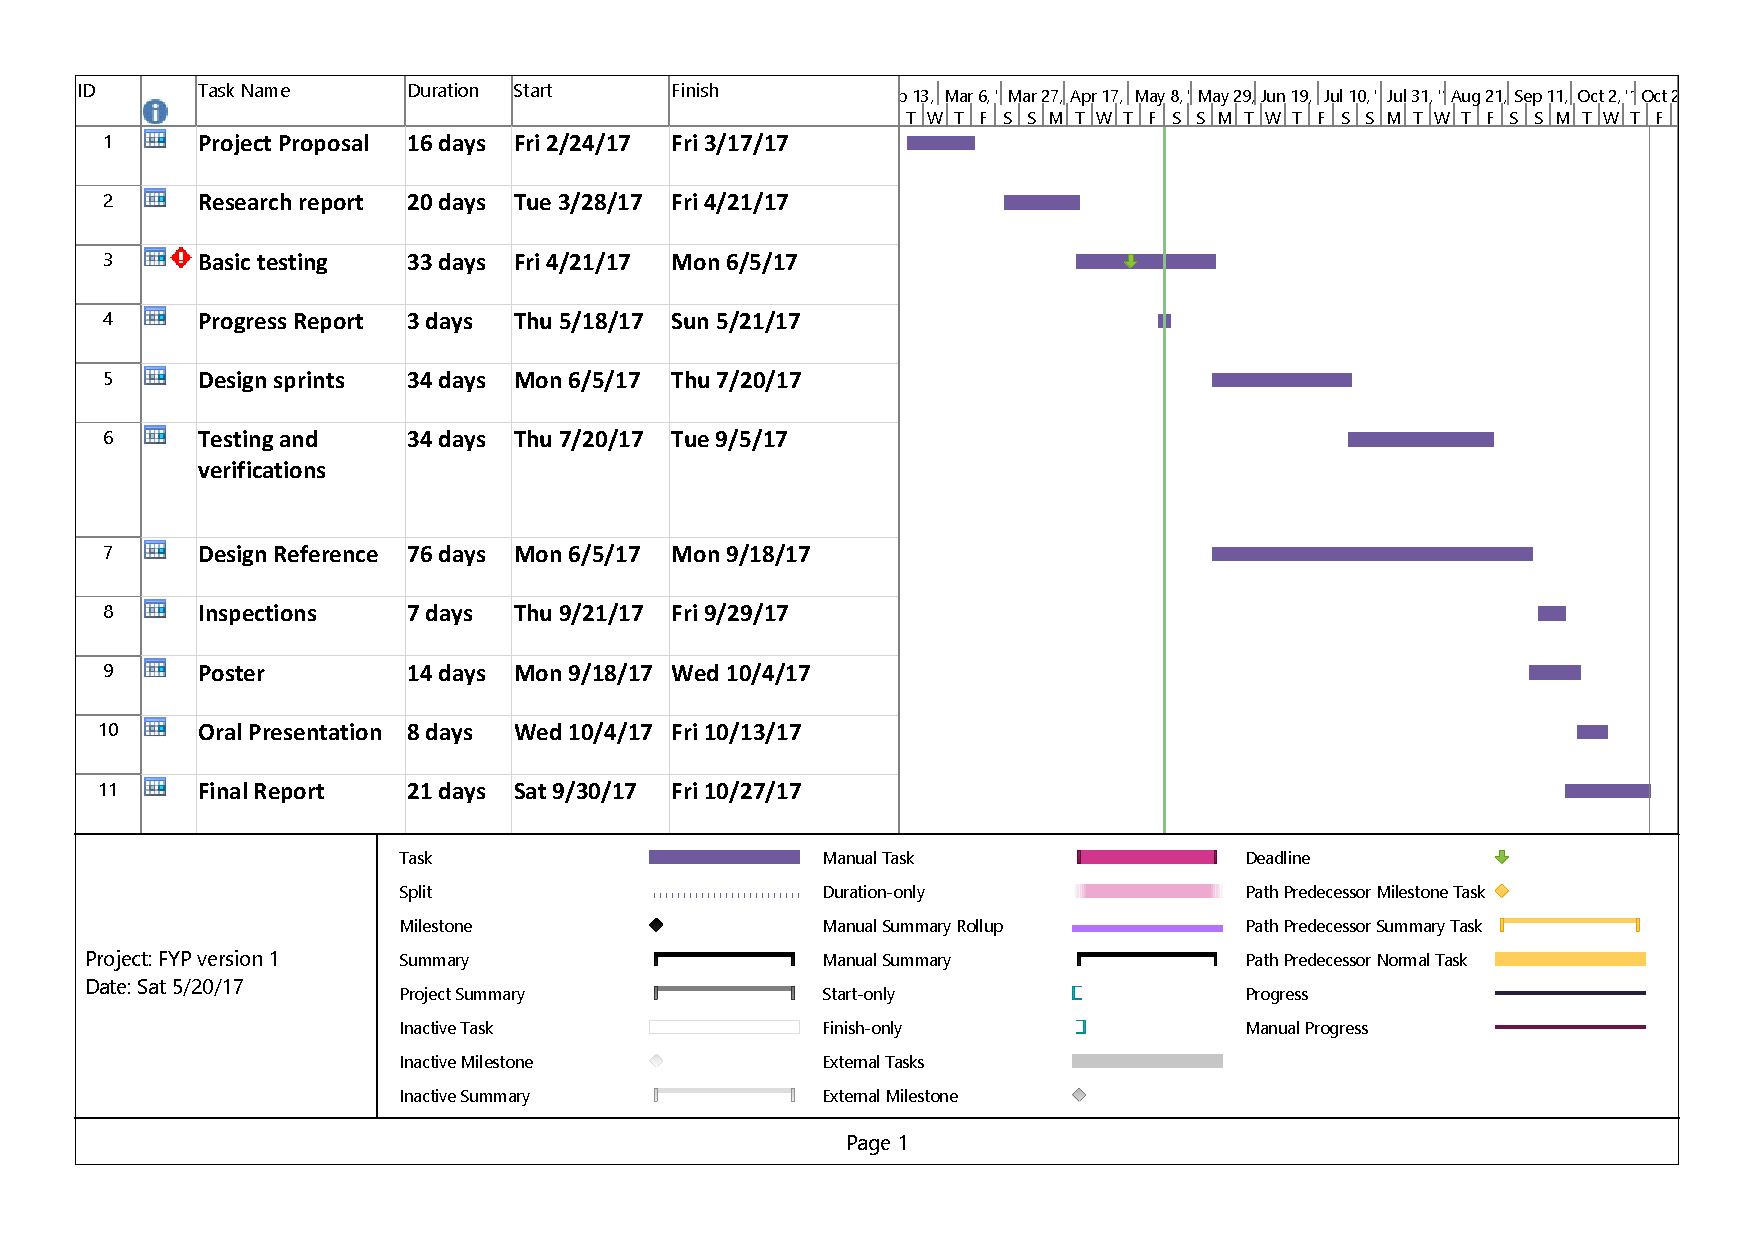
\includegraphics[scale=0.5]{gnattchart2.pdf}
\raggedright

\clearpage
\section{Sustainability Analysis}
\clearpage
\section{Budget Summary}

Table \ref{table:purchases} shows the items the group has felt necessary for our project. We have received all items in this table and have ordered no more. 

\begin{table}[h!]
\centering
\caption{Price of items purchased as of 20/05/2017}
\begin{tabular}{||c|c|c|c||} 
 \hline
 Item & Qty & Price\\
 \hline
 \hline
 LoPy IoT LoRa WiFi BLE development board & 2 & \$96.62 \\
 \hline
 Pycom universal antenna kit & 2 & 40.00\\
 \hline 
 Pycom Universal Expansion board 2.0 & 1 & \$37.50 \\ 
 \hline
  & Total &  174.12\\ 
 \hline
\end{tabular}
\label{table:purchases}
\end{table}
\raggedright




\clearpage

\section{Conclusions}
\clearpage
\section{References}

\end{document}